\documentclass[../TDE1-E2.tex]{subfiles}%

\begin{document}
\section[s]"1"{Calcul de résistances équivalentes}
\QR{%
  Exprimer la résistance équivalente entre les points $A$ et $B$ pour chacun des
schémas suivants.
\bigbreak
\begin{minipage}{0.32\linewidth}
  \begin{center}
    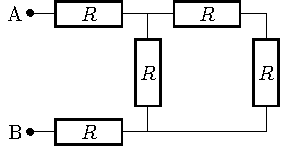
\includegraphics[width=\linewidth]{requiv_a-plain}
  \end{center}
\end{minipage}
\begin{minipage}{0.32\linewidth}
  \begin{center}
    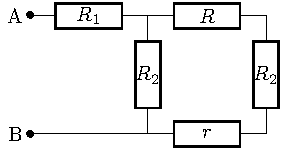
\includegraphics[width=\linewidth]{requiv_b-plain}
  \end{center}
\end{minipage}
\begin{minipage}{0.32\linewidth}
  \begin{center}
    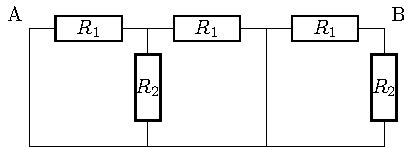
\includegraphics[width=\linewidth]{requiv_c-plain}
  \end{center}
\end{minipage}
}{%
  % \vspace{-30pt}
\subsection{Schéma 1}
\begin{center}
    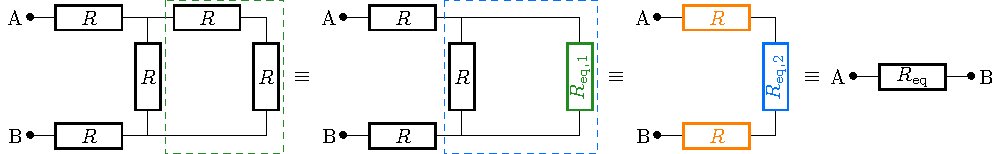
\includegraphics{requiv_a}
\end{center}
La suite de schémas équivalents précédents donne~:
\begin{align*}
    R_{\rm eq}                 & = \textcolor{orange}{R + R} +
        \textcolor{brandeisblue}{R_{\rm eq,2}} \\
    \Leftrightarrow R_{\rm eq} & = \textcolor{orange}{2R} +
        \textcolor{brandeisblue}{\frac{
                R\times \textcolor{ForestGreen}{R_{\rm eq,1}}
        }{R + \textcolor{ForestGreen}{R_{\rm eq,1}}}}\\
    \Leftrightarrow R_{\rm eq} & = 2R + \frac{
        R\times\textcolor{ForestGreen}{2R}}{
        R+\textcolor{ForestGreen}{2R}} \\
    \Leftrightarrow R_{\rm eq} & = 2R + \frac{2R^{\cancel{2}}}{3\cancel{R}}\\
    \Leftrightarrow R_{\rm eq} & = \frac{8R}{3}
\end{align*}

\subsection{Schéma 2}
\begin{center}
    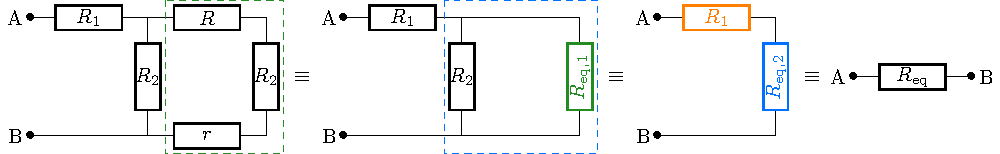
\includegraphics{requiv_b}
\end{center}
Et cette fois~:
\begin{align*}
    R_{\rm eq}                 & =
    \textcolor{orange}{R_1} + \color{brandeisblue}R_{\rm eq,2} \\
    \Leftrightarrow R_{\rm eq} & =
        R_1 + \textcolor{brandeisblue}{\frac{
        R_2\times \textcolor{ForestGreen}{R_{\rm eq,1}}}{
        R_2 + \textcolor{ForestGreen}{R_{\rm eq,1}}}} \\
    \Leftrightarrow R_{\rm eq} & =
        R_1 + \frac{R_2\times(r+R+R_2)}{r+R+2R_2}\\
\end{align*}

\subsection{Schéma 3}
Ce schéma est un peu plus compliqué, mais la bonne pratique de nommer des points
de potentiel sur un schéma aide à ne pas se perdre. En effet, étant donné que
l'on nous demande de déterminer la résistance équivalente entre A et B, toute
simplification du circuit est à faire. On a travaillé sur les associations de
résistances mais il ne faut pas oublier, et donc savoir reconnaître, les
potentiels court-circuits. Ici, en reportant le point A sur chaque point
d'intérêt où il peut être reporté (c'est-à-dire s'il n'y a pas de dipôle entre
les deux), on voit qu'un courant qui partirait de A pour aller à B (ce que fait
un Ohmmètre) éviterait complètement les trois premières résistances. On peut
redessiner le schéma différemment pour faire apparaître le court-circuit de
manière plus explicite~:

\begin{center}
    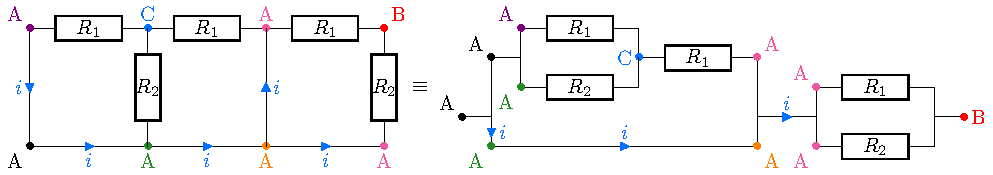
\includegraphics{requiv_c}
\end{center}

Ainsi, le circuit se simplifie en~:
\begin{center}
    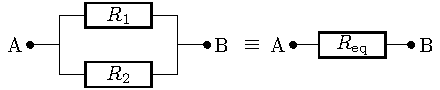
\includegraphics{2parrequiv}
\end{center}
Soit
\[ \boxed{R_{\rm eq} = \frac{R_1R_2}{R_1 + R_2}}\]
}

\end{document}
